\chapter{Mendix} \label{ch:mendix}
    Έχοντας πλέον μια καλή εικόνα για τον ορισμό του χαμηλού κώδικα και των Πλατφόρμων Ανάπτυξης Λογισμικού σε Low-Code, στο παρόν κεφάλαιο, θα επικεντρωθούμε σε μια από αυτές τις πλατφόρμες, το Mendix, η οποία αποτέλεσε το βασικό εργαλείο για την υλοποίηση της εφαρμογής που αναπτύχθηκε στο πλαίσιο της παρούσας διπλωματικής εργασίας. Θα...

%Σε αυτό το κεφάλαιο, θα παρουσιαστούν αναλυτικά οι βασικές λειτουργίες και τα χαρακτηριστικά της πλατφόρμας, καθώς και οι λόγοι που την καθιστούν κατάλληλη για την ανάπτυξη της συγκεκριμένης εφαρμογής. Επιπλέον, θα αναλυθούν τα εργαλεία που χρησιμοποιήθηκαν, οι τεχνολογίες που υποστηρίζει και τα πλεονεκτήματα που προσφέρει σε σχέση με άλλες παρόμοιες πλατφόρμες.

    \section{Τι είναι το Mendix;}
        Το Mendix αποτελεί μία από τις πιο διαδεδομένες πλατφόρμες ανάπτυξης λογισμικού που βασίζεται σε χαμηλό κώδικα. Ιδρύθηκε το 2005 στο Ρότερνταμ της Ολλανδίας με στόχο να παρέχει στους επιχειρηματίες και τους οργανισμούς τη δυνατότητα να αναπτύσσουν, να προσαρμόζουν και να διαχειρίζονται εφαρμογές αποδοτικά με χαμηλό κόστος. Το Mendix περιλαμβάνει όλα τα οφέλη και τα χαρακτηριστικά των LCDP που έχουν περιγραφτεί στην ενότητα \ref{sec:LCDP}, συμπεριλαμβάνοντας γραφικό περιβάλλον με WYSIWYG GUI σχεδιαστή, drag-and-drop εργαλεία και έτοιμες βιβλιοθήκες, τη χρήση domain models, το εύκολο deployment της εφαρμογής στο clout, version control μέσω Git, συνεργασία χρησιμοποιώντας Agile μεθοδολογία και άλλα.

        Το 2018, το Mendix εξαγοράστηκε από τη Siemens, τη μεγαλύτερη βιομηχανική κατασκευαστική εταιρεία στην Ευρώπη, γεγονός που επέφερε σημαντικές εξελίξεις στην πλατφόρμα. Η συγχώνευση αυτή επέτρεψε την ενσωμάτωση προηγμένων βιομηχανικών και IoT (Internet of Things) λύσεων, ενισχύοντας τη θέση του Mendix στην αγορά των λογισμικών σχεδιασμένων για επιχειρήσεις. Έτσι, το Mendix αποτελεί μία από τις πιο ισχυρές και ευέλικτες λύσεις στην αγορά του low-code προγραμματισμού, προσφέροντας αποτελεσματικότητα, ταχύτητα και καινοτομία στην ανάπτυξη λογισμικού, ενώ παράλληλα ενσωματώνει τις πιο σύγχρονες τεχνολογίες για να καλύψει τις ανάγκες επιχειρήσεων που επιθυμούν να παραμείνουν ανταγωνιστικές στην ψηφιακή εποχή. \cite{LowCodeMendix}

        Η Gartner, μία από τις μεγαλύτερες εταιρείες έρευνας και συμβουλευτικής στον κλάδο της τεχνολογίας, χαρακτηρίζει το Mendix ως ηγέτη στην αγορά των πλατφορμών ανάπτυξης λογισμικού για 8 συνεχόμενα χρόνια, (βλ. Σχήμα \ref{fig:GartnerQuadrant}). Η κατάταξη αυτή αποδεικνύει την ικανότητα του Mendix να παρέχει λύσεις υψηλής ποιότητας και αξίας στους πελάτες του, καθώς και την ικανότητά του να προσαρμόζεται στις ανάγκες της αγοράς και να προσφέρει συνεχώς καινοτόμες λύσεις. \cite{mendixGartnerQuadrant} Για αυτούς τους λόγους έχει προτιμηθεί για την υλοποίηση της εφαρμογής που θα παρουσιαστεί στο επόμενο κεφάλαιο.

            \begin{figure}[h!] \noindent \centering
                    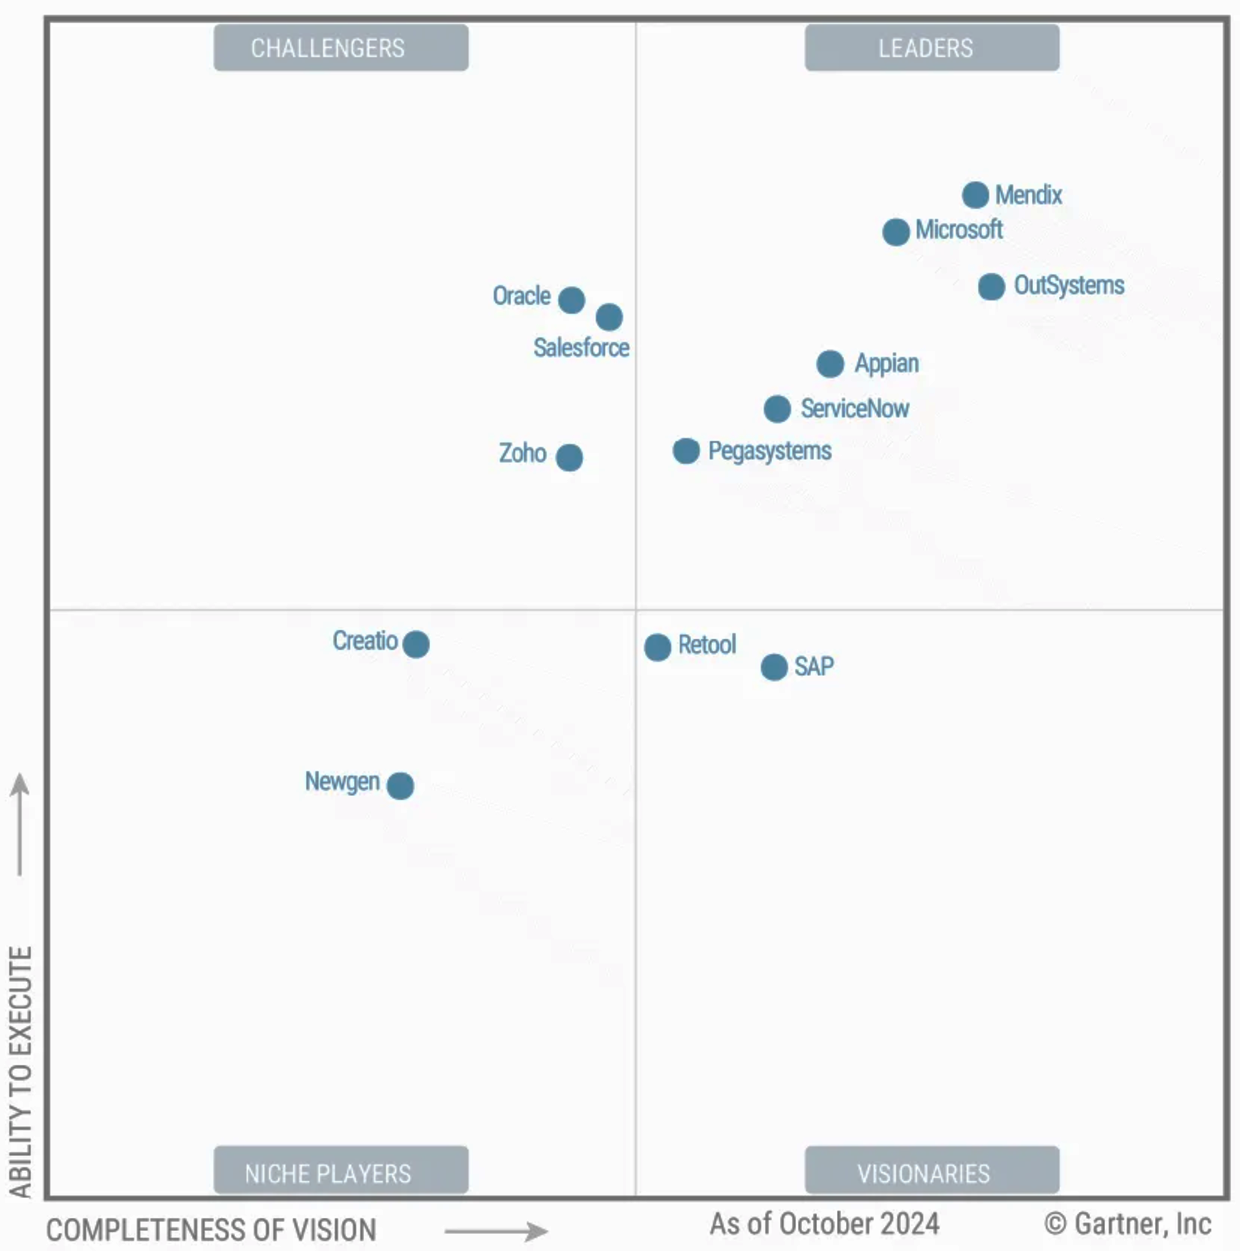
\includegraphics[width=0.5\textwidth]{GartnerQuadrant}
                    \caption{\centering Τεταρτημόριο της Gartner με πλατφόρμες ανάπτυξης λογισμικού \cite{mendixGartnerQuadrant}}
                    \label{fig:GartnerQuadrant}
            \end{figure}

    \section{Το Mendix Studio}
        Το Mendix Studio Pro επιτρέπει τη δημιουργία, προβολή και την ανάπτυξη εφαρμογών στην πλατφόρμα Mendix.

        \begin{figure}[h!] \noindent \centering
                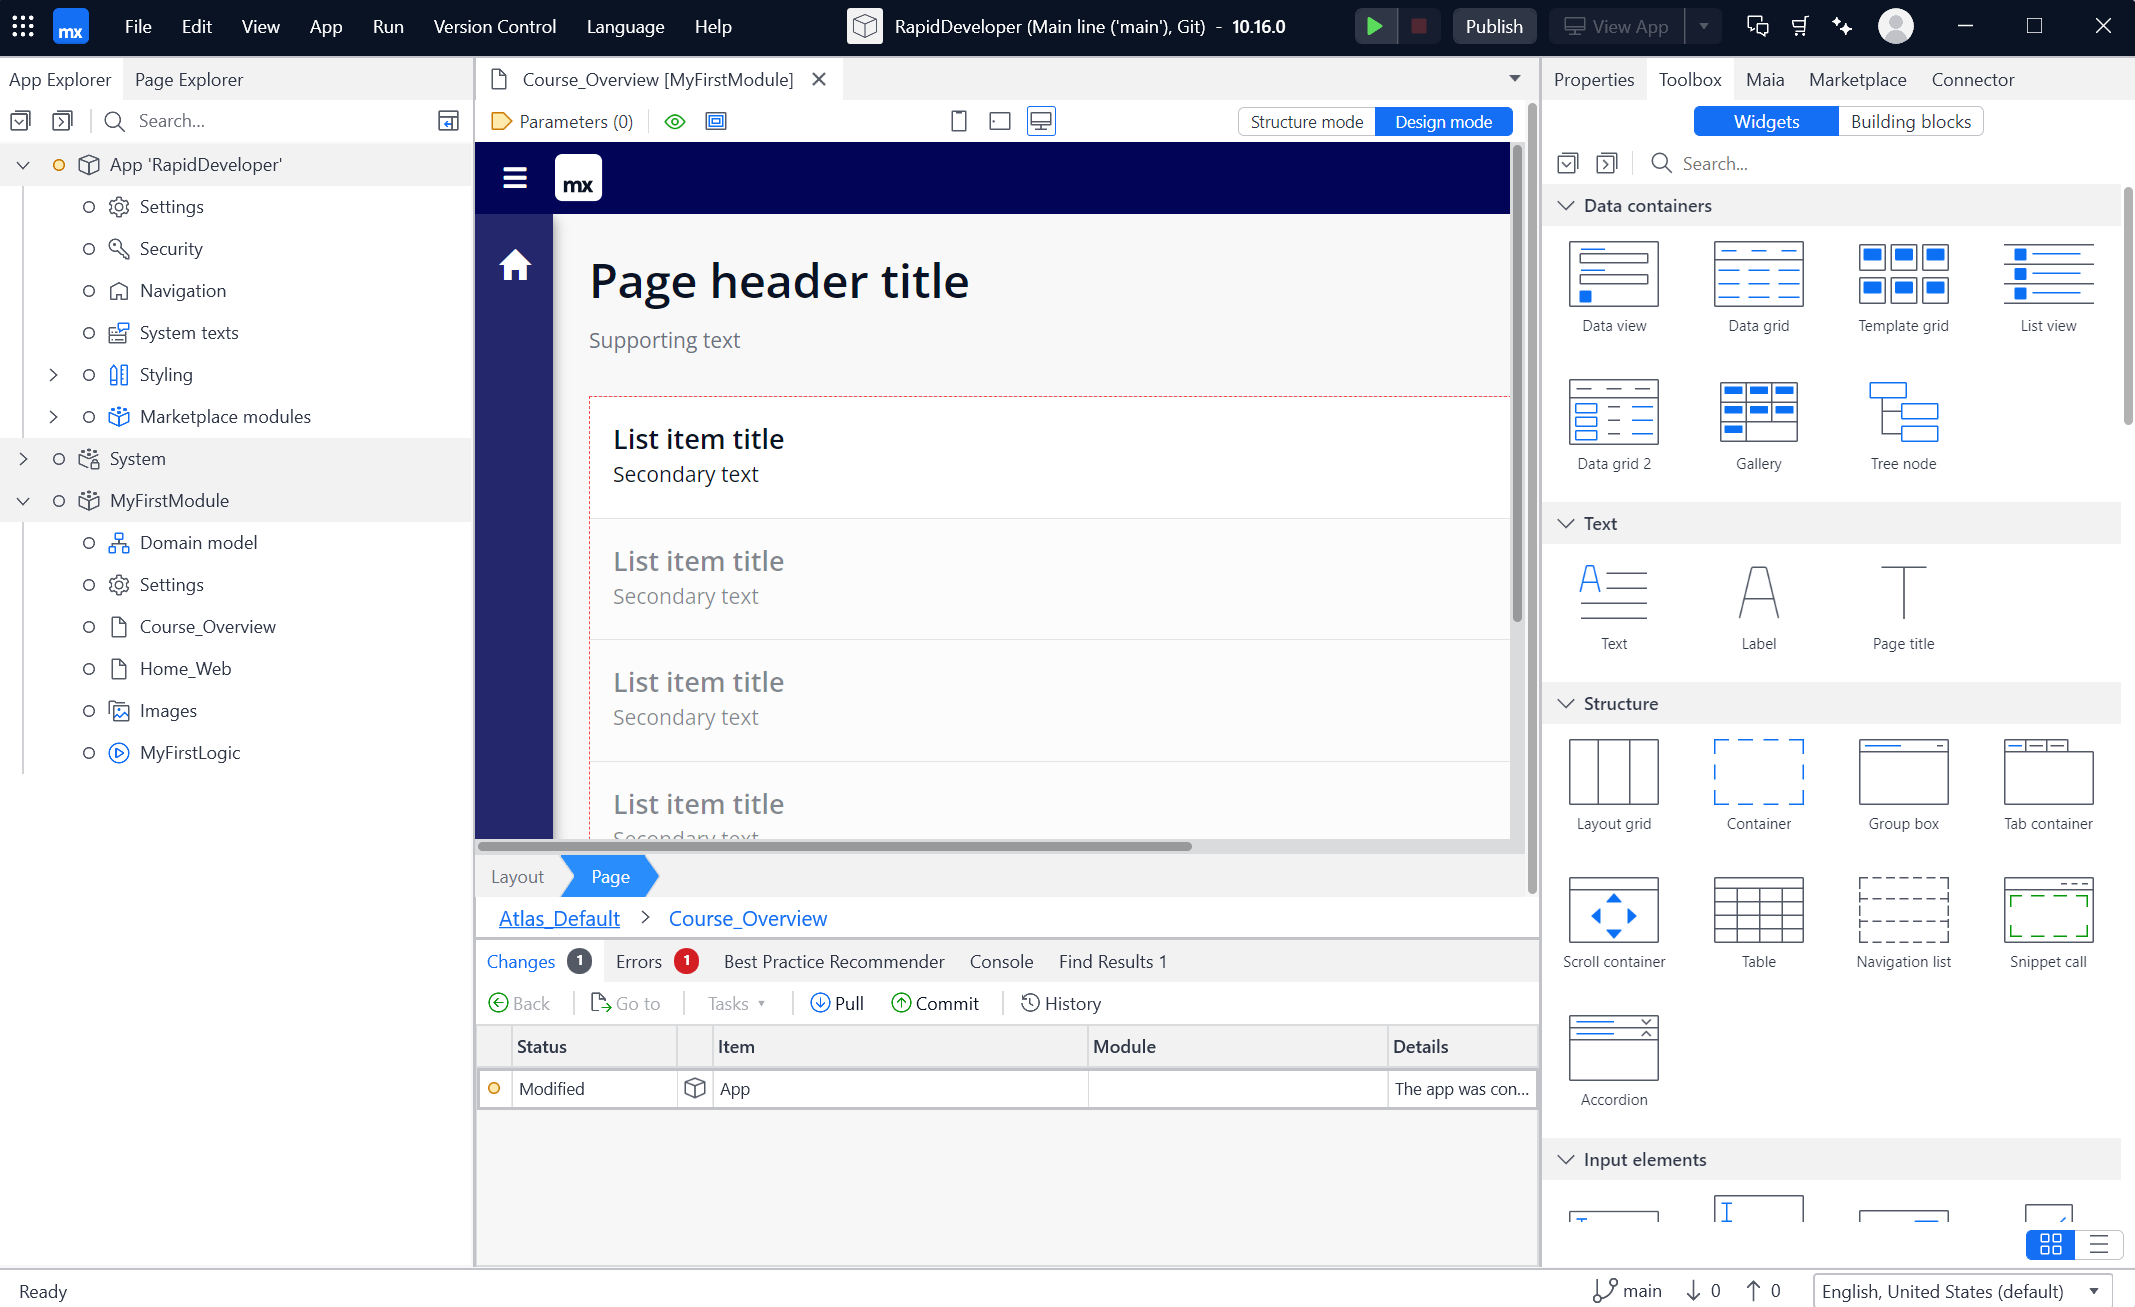
\includegraphics[width=\textwidth]{Mendix/MendixStudioOverlay}
                \caption{\centering Στιγμιότυπο του Mendix Studio Pro.}
                \label{fig:MendixStudioOverlay}
        \end{figure}

        \subsection{Περιβάλλον ανάπτυξης}
        Στο \ref{fig:MendixStudioOverlay} παρουσιάζεται το γραφικό περιβάλλον του Mendix Studio Pro με ανοιχτή την εφαρμογή \say{RapidDeveloper}\footnote{Η εφαρμογή RapidDeveloper δημιουργήθηκε ως αποτέλεσμα των μαθημάτων (crash courses) που προσφέρονται μέσω του Mendix Academy. Αυτά τα μαθήματα έχουν σχεδιαστεί για να παρέχουν στους χρήστες μια γρήγορη και πρακτική εισαγωγή στις βασικές δυνατότητες της πλατφόρμας Mendix, επιτρέποντάς τους να εξοικειωθούν με τη διαδικασία ανάπτυξης εφαρμογών σε περιβάλλον low-code.}.

        Μπορούμε να διαχωρίσουμε το γραφικό περιβάλλον σε τέσσερα μέρη. Η μαύρη μπάρα στο πάνω μέρος περιλαμβάνει το βασικό μενού του λογισμικού, το όνομα της εφαρμογής που αναπτύσσουμε, κουμπιά τα οποία επιτρέπουν είτε την τοπική εκτέλεση της εφαρμογής μέσω localhost ή τη διάθεσή της στο cloud, στο \textit{Mendix Sandbox}, και σύνδεσμοι που οδηγούν στο Mendix προφίλ του χρήστη, στο Marketplace κ.α.

        Στο κεντρικό τμήμα της οθόνης, κάτω από την επάνω μπάρα, βρίσκεται το \textit{Working Area}, όπου εμφανίζονται οι σελίδες της εφαρμογής μας. Στην αριστερή πλευρά, εντοπίζουμε τον \textit{App Explorer}, ο οποίος περιλαμβάνει τη δομή φακέλων και αρχείων της εφαρμογής, καθώς και τον \textit{Page Explorer}, που καταγράφει όλα τα στοιχεία που έχουν χρησιμοποιηθεί στη σελίδα της εφαρμογής που είναι ανοιχτή. Στη δεξιά πλευρά, βρίσκεται το \textit{Properties} Panel, όπου εμφανίζονται όλες οι ρυθμίσεις και οι παράμετροι των επιλεγμένων στοιχείων, και το \textit{Toolbox}, το οποίο περιέχει ένα σύνολο από προκατασκευασμένα στοιχεία που μπορούν να εισαχθούν στην εφαρμογή. Στο κάτω μέρος εμφανίζονται panels με τις αλλαγές που πραγματοποιούμε ανά commit, τα σφάλματα που υπάρχουν, logs, κονσόλα και άλλα. Μπορούμε σε οποιαδήποτε πεδίο να προσθέσουμε ή να αφαιρέσουμε Panels από το $ \text{Μενού} \rightarrow \text{View} $. \cite{mendixDoc}

        \subsubsection{Επιλογές για deployment} \label{sec:MendixDeployment}
            Το Mendix παρέχει διάφορες επιλογές για το deployment των εφαρμογών που αναπτύσσονται στην πλατφόρμα.

            Το Mendix Free δημιουργεί ένα δωρεάν online sandbox το οποίο επιτρέπει τη δημόσια διάθεση της αναπτυσσόμενης εφαρμογής. Το Mendix Free είναι κατάλληλο για την ανάπτυξη μικρών εφαρμογών και την εξοικείωση με την πλατφόρμα, αλλά δεν προσφέρει την απαιτούμενη ασφάλεια και ευελιξία για την ανάπτυξη μεγάλων επιχειρησιακύν εφαρμογών καθώς οι εφαρμογές παύουν να λειτουργούν μετά από λίγες ώρες αδράνειας (sleep mode), δεν μπορούν να κλιμακωθούν, υπάρχει όριο στην υπολογιστική ισχύ και το μέγεθος της βάσης δεδομένων, δεν τρέχουν προγραμματιζόμενα γεγονότα, δεν υποστηρίζονται custom domains κ.α. Παρόλα αυτά είναι μια πολύ καλή επιλογή που εξυπηρετεί τις ανάγκες των αρχάριων χρηστών και μικρών εφαρμογών. \cite{mendixCloud}

            Για χρήστες ή επιχειρήσεις με αυξανόμενες ανάγκες, το Mendix προσφέρει λύσεις επί πληρωμή που άρουν τους περιορισμούς που αναφέρθηκαν νωρίτερα.


    \section{Δομή εφαρμογών του Mendix}
        Μια εφαρμογή στο Mendix απαρτίζεται από διαφορετικά έγγραφα και modules.

        Τα modules ουσιαστικά διαχωρίζουν τη λειτουργικότητα της εφαρμογής σε αυτοτελή κομμάτια. Ο τρόπος με τον οποίο πραγματοποιείται ο διαχωρισμός εξαρτάται από την κρίση και τη σχεδιαστική προσέγγιση του μηχανικού λογισμικού. Μια εφαρμογή περιλαμβάνει ένα \textit{System} module, modules που καθορίζονται από τους χρήστες ή modules από το Marketplace του Mendix, τα οποία μπορούν να προσφέρουν επιπλέον λειτουργικότητες κατασκευασμένες από τρίτους. Τέλος, μπορούμε να ορίσουμε modules με μοναδικό σκοπό τον καθορισμό της εμφάνισης της εφαρμογής (UI resources modules). Αυτά εμφανίζονται με πράσινο χρώμα και περιλαμβάνουν πρότυπα σελίδων (page templates) και δομικά στοιχεία (building blocks).

        Για παράδειγμα, στο App Explorer της εφαρμογής RapidDeveloper (σχήμα \ref{fig:MendixStudioOverlay}) παρατηρούμε πως εμφανίζονται τρία διαφορετικά modules: το module App, το module \say{System} και το module {MyFirstModule}. Τα δύο πρώτα είναι modules που δημιουργούνται αυτόματα κατά τη δημιουργία μιας εφαρμογής, ενώ το τρίτο είναι ένα module που δημιουργήθηκε από τον χρήστη.

        Στο module App μπορούν να επεξεργαστούν γενικές ρυθμίσεις που αφορούν την εφαρμογή. Συγκεκριμένα σε κάθε εφαρμογή του Mendix αντιστοιχούν πλαίσια διαλόγου για τις Ρυθμίσεις (Settings) της εφαρμογής, την Ασφάλεια (Security), την Πλοήγηση (Navigation), τα Κείμενα Συστήματος (System Texts)\footnote{Στο έγραφο με τα Κείμενα Συστήματος μπορεί να γίνει μετάφραση των μηνυμάτων που παράγονται από τον διακομιστή κατά την εκτέλεση μιας εφαρμογής (για παράδειγμα \say{Password too short}).} και την Εξαγωγή Documentation (Export Documentation)\footnote{Στην Εξαγωγή Documentation μπορεί να εξαχθεί ένα HTML αρχείο με τα έγγραφα της εφαρμογής και το αντίστοιχο documentation.}.

        Οι Ρυθμίσεις περιλαμβάνουν παραμετροποιήσεις για το runtime της εφαρμογής, το theme που χρησιμοποιείται, την επιλογή ενεργειών (microflows) πριν αρχικοποιηθεί η εφαρμογή κατά την εκκίνησή της, επιλογή hash αλγορίθμων, γλώσσας κα.

        \begin{figure}[h!] \noindent \centering
                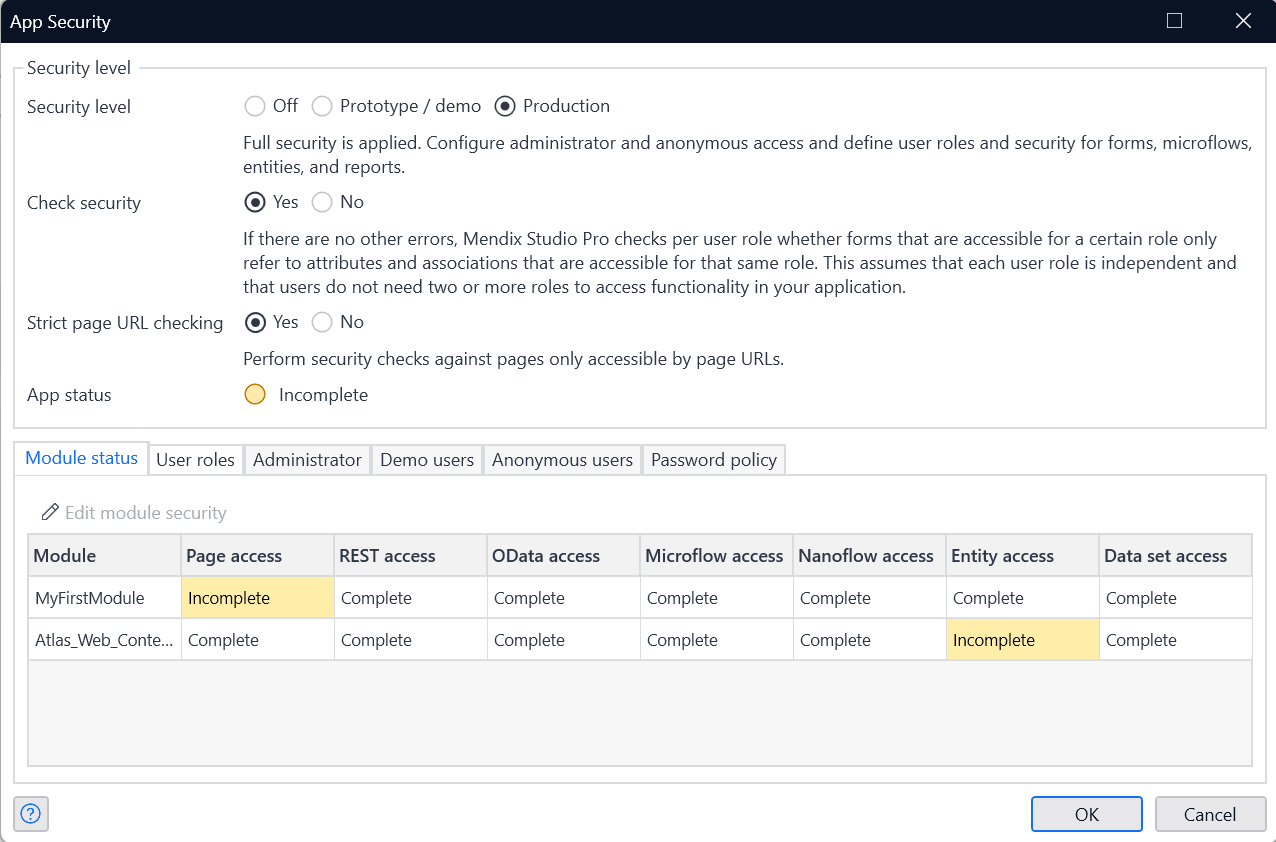
\includegraphics[width=0.8\textwidth]{Mendix/AppSecurity}
                \caption{\centering Παράθυρο App Security.}
        \end{figure}

        Στην Ασφάλεια μπορούν να τροποποιηθεί το επίπεδο ασφάλειας (security level) της εφαρμογής (μπορεί να επιλεγεί ώστε οι χρήστες να μη χρειάζεται να συνδεθούν για να έχουν πρόσβαση ή να χρειάζεται σύνδεση), μπορούν να οριστούν ρόλοι χρηστών (δημιουργούνται ρόλοι στους χρήστες όπως Administrator, User, Guest και ανατίθενται τα modules και οι σελίδες στα οποία επιτρέπεται να έχουν πρόσβαση), διαπιστευτήρια του διαχειριστή της εφαρμογής (Adminstrator), ορίζονται demo χρήστες, ανώνυμοι χρήστες (οι οποίοι έχουν πρόσβαση στην εφαρμογή χωρίς να συνδεθούν) και να ρυθμιστούν κανόνες για τους κωδικούς πρόσβασης.

        \begin{figure}[h!] \noindent \centering
                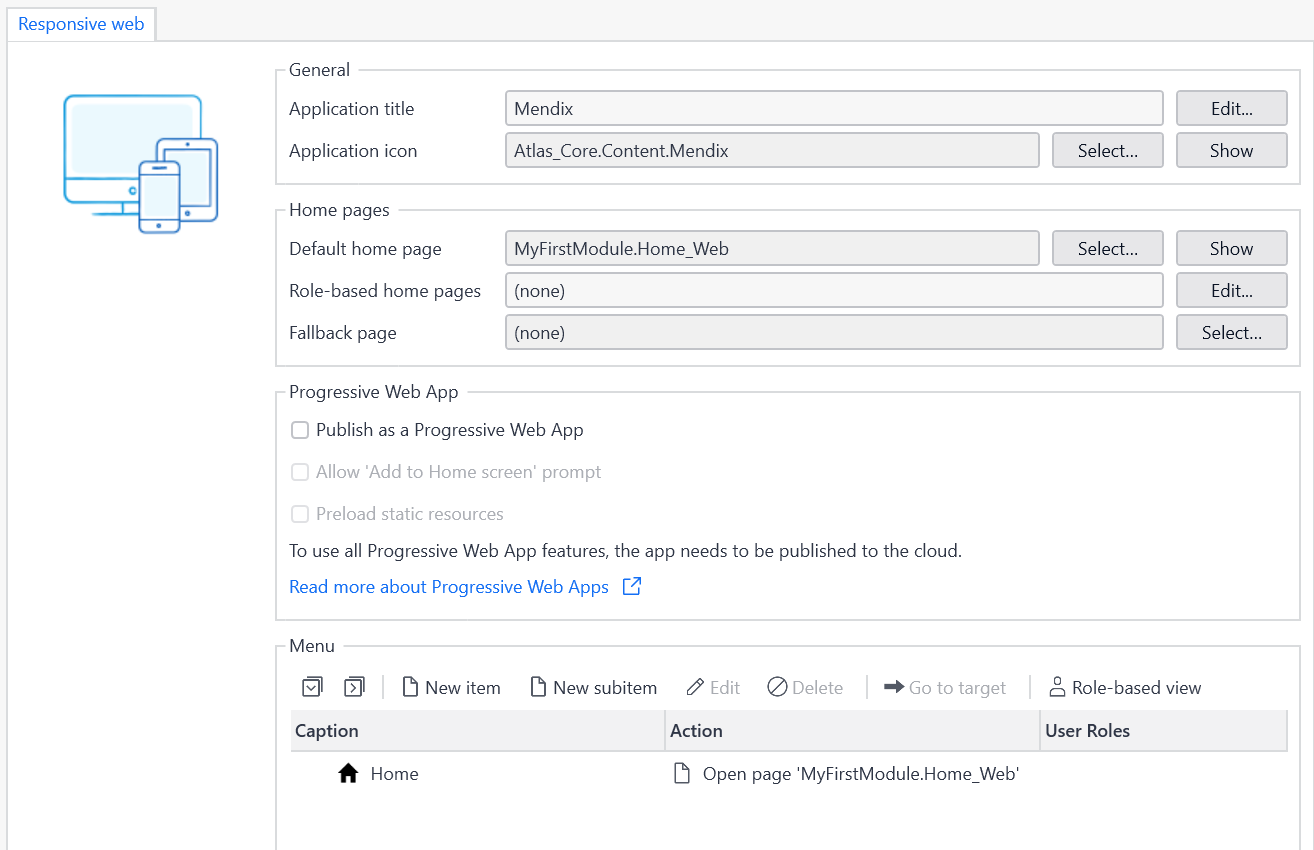
\includegraphics[width=0.8\textwidth]{Mendix/Navigation}
                \caption{\centering To έγγραφο Navigation.}
        \end{figure}

        Στην Πλοήγηση μπορούν να διαμορφωθούν το όνομα και το εικονίδιο της εφαρμογής, η μπάρα μενού και η δομή του δέντρου πλοήγησης (navigation tree) και η αρχική σελίδα (home page) της εφαρμογής, η οποία μπορεί να είναι διαφορετική για κάθε ρόλο χρήστη.

        Η Πλοήγηση είναι ένα \textit{έγγραφο} της εφαρμογής. Άλλα παραδείγματα εγγράφων είναι οι Σελίδες, τα Microflows, τα Enumerations, οι Εικόνες και τα Layouts.

